\section{Morpheus}

\subsection{Descrição}
%TODO add source below
Morpheus é o servidor local responsável pela interconexão da casa inteligente com os serviços de nuvem. O nome tem sua origem na mitologia grega, onde o Deus dos sonhos, Morpheus, era responsável pelo envio de mensagens entre dois mundos diferentes, o dos deuses e o dos mortais [add source]. Sua principal atribuição é garantir que a troca de mensagem entre os módulos e a nuvem seja realizada com segurança e confiabilidade, munindo-se de soluções robustas para desempenhar o seu papel.

\subsection{Plataforma}
O Morpheus tem seu desenvolvimento realizado em Java. Conforme será detalhado em seguida, tal escolha foi realizada com base na portabilidade que a máquina virtual Java (JVM) oferece, bem como na disponibilidade de bibliotecas e serviços largamente utilizados em aplicações comerciais. O servidor foi construído utilizando-se o Spring Boot Framework, com a utilização de seu container de Inversão de Controle (\textit{IoC - Inversion of Control}), para injeção de dependências. Essa técnica diminui o acoplamento entre classes, e permite a evolução e implementação de novas funcionalidades de maneira mais facilitada.

Para se comunicar com os módulos, o Morpheus utiliza-se da conexão com um broker \wmqtt{}, o qual utilizamos o Mosquitto, por ser uma solução Open Source largamente utilizada em projetos de Internet of Things. Conforme detalhado a frente, configurações de segurança específicas para nosso projeto foram registradas no broker. Para a conexão com os serviços na nuvem, é utilizado um canal Websocket, aberto pelo Morpheus (cliente) e aceito pela nuvem (servidor). Esta solução veio a partir de uma discussão em relação à segurança, a qual está documentada aqui. Na figura a seguir, é possível verificar a arquitetura desenvolvida.

\subsection{Tecnologias utilizadas}
Toda a implementação do Morpheus foi realizada em java. Desde o começo do projeto, decidiu-se que a escolha de tecnologias para implementação das diversas camadas deveria ter por base os seus benefícios, e não necessitaria ser rígida ou uniforme. Assim, o principal esforço foi sempre no planejamento das interfaces de comunicação entre as partes, que poderiam ser desenvolvidas em linguagens complementamente diferentes. Os sistemas de nuvem, por exemplo, foram implementados em Node.js, com front-end em React. Os módulos de hardware foram programados em C e, como comentado acima, o controlador local em Java.
Essa flexibilidade permitiu com que fossem utilizados os recursos e tecnologias que fossem melhores integrados com os requisitos propostos.

Um requisito essencial para o controlador local é a sua robustez. Em um cenário em que este controlador não esteja disponível, a casa passa a funcionar em estado de emergência, onde os comandos são reduzidos, e não permitem acesso remoto. Entretanto, há inúmeras possibilidades e eventos que poderiam causar a queda deste controlador, muitas das quais referem-se a situações fora de nosso alcance. A falta de energia na residência, ou de internet, interrompe o seu funcionamento, e não é possível ter controle sobre tal situação. O mesmo ocorre no evento de problemas de hardware, na plataforma que o sistema estiver rodando. Ao mesmo tempo que tais situações estejam fora de nosso controle, os planos para contenção dos seus efeitos são complexos, custosos e fogem do escopo deste projeto, como seria o caso de se implementar duplicações, banco de baterias e tecnologia celular para comunicação secundária.

Há, entretanto, problemas no software que poderiam afetar o funcionamento do controlador. Por meio de testes, muitos desses problemas podem ser evitados, ainda em tempo de desenvolvimento. A utilização de tecnologias que facilitam o desenvolvimento seguro da aplicação é uma vantagem para este caso, já que ferramentas estão disponíveis para que haja maior controle sobre o código desenvolvido, e a pode-se detectar erros mais facilmente, ainda em tempo de compilação, por exemplo.
O controlador local também precisa lidar com as requisições assíncronamente. Parte desta tarefa é facilitada, com a utilização do sistema de mensageria \wmqtt{}, operado pelo Broker Mosquitto. Com sua utilização, mensagens podem ser enviadas, e mesmo que o controlador não consiga recebê-las, elas não serão perdidas. Entretanto, devido às características do sistema proposto, as mensagens precisam ser operadas sem maiores demoras. O controlador deve receber e processar as mensagens paralelamente, e não esperar o processamento de uma mensagem inteira, para assim processar a próxima, de modo que paralelismo deve ser parte essencial da arquitetura.

Ainda, para a integração com os serviços da nuvem, é necessário a utilização de JSON, para a serialização das mensagens, em um formato que pode ser desserializado posteriormente, independentemente da plataforma. Para a utilização de WebSockets, é necessário o uso de bibliotecas disponíveis, de modo que o desenvolvimento seja facilitado. Por último, é necessário gerenciar eficientemente todas essas dependências. Atualizá-las quando necessário, ou substituí-las, se desejado, deve ser uma tarefa simples.

A arquitetura oferecida pelo Java mostra ser efetiva para as necessidades levantadas acima. Com a utilização de uma IDE avançada, inúmeros recursos estão disponíveis para limpeza, refatoração, organização do código, etc. O \textit{framework} Spring Boot\footnote{https://projects.spring.io/spring-boot/} foi utilizado para o desenvolvimento, por oferecer diversos recursos que facilitam o desenvolvimento, com configurações de ambiente e o oferecimento de um container para inversão de controle e injeção de dependência\footnote{https://martinfowler.com/articles/injection.html}. Além disso, o gerenciador de dependências Gradle\footnote{https://gradle.org/} foi também utilizado, por oferecer um poderoso ambiente para configurar, construir e distribuir aplicações. Gradle faz uso de Groovy\footnote{http://groovy-lang.org/}, tecnologia que também roda na \textit{Java Virtual Machine} (JVM). Por outro lado, o uso de tais ferramentas e plataformas necessita de hardware mais robusto, para que funcione, sendo uma desvantagem. Entretanto, frente aos benefícios, ainda é vantajoso a utilização de Java, neste caso.

Java é utilizado em vasta gama de aplicações, deste complexos softwares comerciais como a IDE Eclipse, até software embutidos, como controladores de BlueRay\footnote{http://www.oracle.com/technetwork/articles/javame/bluray-142687.html}.
O padrão de inversão de controle, com injeção de dependências, foi utilizado para o desenvolvimento, de modo a diminuir o acoplamento entre as partes, e facilitar futuras modificações. Assim, cada módulo recebe, em seu construtor, todas as dependências que serão utilizadas. A responsabilidade da construção de tais dependências passa, então, a ser responsabilidade do gerenciador de contexto, e não mais do módulo. A escolha do Java 8 foi decidida para que o desenvolvimento possa utilizar certos recursos de paradigmas funcionais, como o conceito de Streams de dados e Funções Lambdas.

Internamente, o Morpheus é dividido em pacotes, que responsáveis pela modelagem do problema. Há classes que modelam o domínio, que executam as regras de negócio, que fazem a interface entre outros sistemas (\wmqtt{} Mosquitto Broker e nuvem), e também para execução de tarefas como backup de mensagens, e serviços de conversão.
Assim que uma mensagem chega ao Morpheus, ela é reconhecida e é realizado o seu parsing, para as estruturas de domínio internas. Caso haja algum erro, para mensagens vindas da nuvem, há o envio de relatório com os problemas encontrados. A partir daí, a mensagem é colocada em uma fila interna, onde outro módulo será responsável por capturá-la e realizar o processamento necessário.

\begin{figure}
	\centering
	\caption{Arquitetura do servidor local}
  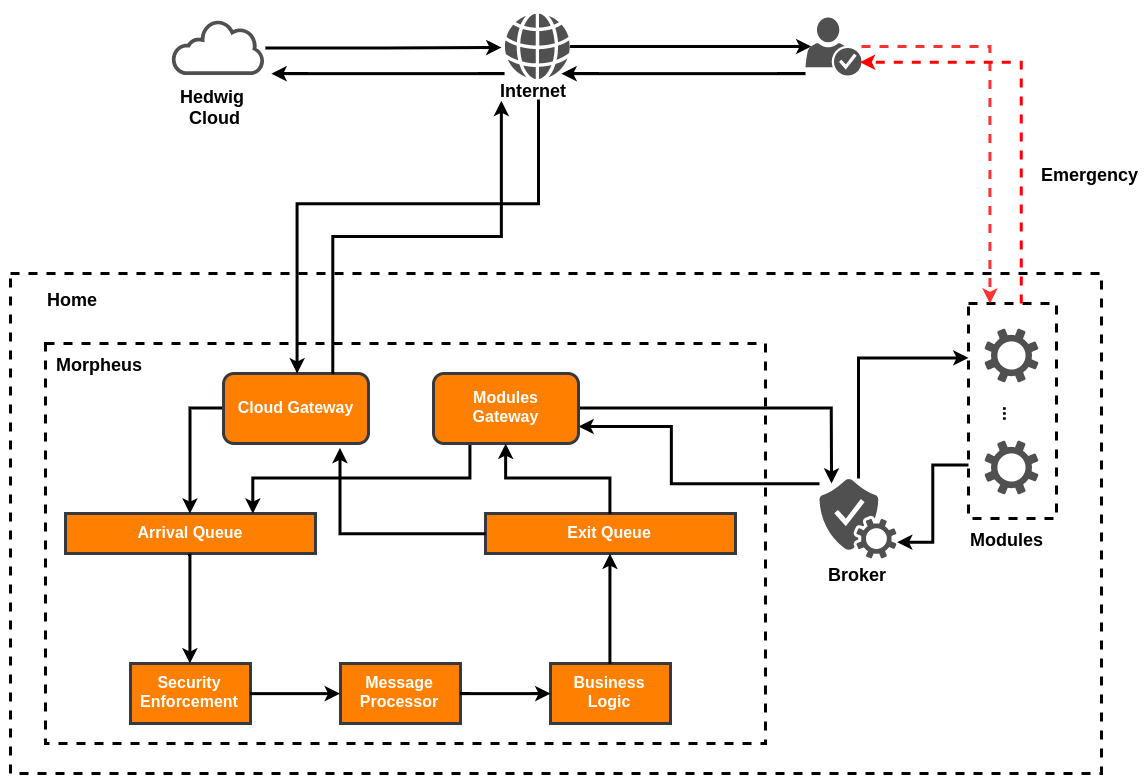
\includegraphics[width=\textwidth]{diagramaDeComunicacao}
\label{fig:diagramaDeComunicacao}
\end{figure}

\subsection{Requisitos}
Para a concepção do servidor local, foram discutidos os seus requisitos funcionais e não funcionais, bem com suas prioridades na implementação.

\subsubsection{Requisitos Funcionais}
\begin{description}

\item \textbf{Configuração dos módulos}

De acordo com as regras e interfaces estabelecidas, documentadas aqui, os módulos podem ser configurados por meio de mensagens. Os serviços da nuvem enviarão os parâmetros de configuração de cada módulo ao Morpheus, que os transmitirão ao módulo.

\item \textbf{Conexão de emergência}

Quando não há conexão da casa com a nuvem, deverá haver um canal para comunicação local entre o aplicativo e alguns dos módulos, com funcionalidades limitadas, apenas para serviços essenciais.

\item \textbf{Envio de dados para a nuvem}

Dados provenientes de sensores são enviados para a nuvem, para que sejam tratados de acordo com as regras de Business Intelligence, por meio de Machine Learning.

\item \textbf{Persistência de dados}

Quando não houver conexão, o servidor deverá armazenar os dados localmente e, quando solicitado, enviá-los à nuvem.

\item \textbf{Tentativas de reenvio}

Quando uma mensagem não é enviada com sucesso à nuvem, o Morpheus deverá tentar novamente, um número configurável de vezes, em um
curto espaço de tempo. Isso ocorre pois, se determinada mensagem não pode ser enviada em uma janela temporal, ela perde o seu sentido, mesmo por questões de segurança.

\item \textbf{Envio de e-mail}

Se o Morpheus estiver desconectado da nuvem por um período, configurável, deverá avisar o usuário, por meio de uma mensagem de e-mail.

\item \textbf{Verificação do time-stamp}

Quando uma nova mensagem chegar, seu timestamp deverá ser verificado, e a mensagem tomará curso somente se não for obsoleta.

\item \textbf{Tomadas de ação}

Quando o usuário requisitar uma tomada de ação, esta deverá ser enviada por meio de uma mensagem ao Morpheus, o qual a transmitirá ao módulo.

\item \textbf{Configuração em arquivo}

As configurações básicas do Morpheus devem ser registradas em um arquivo YAML, que será lido durante a inicialização.

\item \textbf{Listeners para diferentes tipos de mensagens}

Deverão haver listeners para todos os tipos de mensagens, definidos aqui, que serão recebidos da nuvem e dos módulos.

\end{description}

\subsubsection{Requisitos Não Funcionais}
\begin{description}
\item \textbf{Processamento concorrente}

Toda a infraestrutura do Morpheus deverá permitir o processamento de mensagens de maneira concorrente. Não deve ser permitido esperar o processamento completo de uma mensagem para que outra comece a ser processada.

\item \textbf{Utilização de criptografia na troca de mensagens com a nuvem}

Os dados que trafegam entre a nuvem e o servidor local não devem ser codificados em texto puro. Devem estar protegidos contra sniffers.

\item \textbf{Conversão de mensagens}

As mensagens enviadas à nuvem devem estar em formato JSON, e não no protocolo definido aqui, para troca de mensagens entre os módulos e o Morpheus.

\item \textbf{Serialização das configurações}

O servidor deverá serializar e persistir as configurações relativas aos módulos que foram configurados, e carregá-las em sua inicialização.

\item \textbf{Destruição de pools de threads}

Ao ser desligado, todos os pools de threads criados devem ser destruídos.

\end{description}

\subsection{Especificações}

\subsubsection{Tópicos}
Todos os tópicos devem seguir o formato especificado abaixo. Com essa formatação, é possível garantir que:

\begin{enumerate}
\item Somente o Morpheus conseguirá publicar em qualquer tópico, ou ser um subscriber de qualquer tópico.
\item Cada módulo somente consiga publicar no tópico determinado para ele, que será garantido com as credenciais (usuário e senha) fornecidos pelo tópico.
\item Caso um módulo malicioso seja implantado, com o roubo das credenciais de um módulo legítimo, o impacto será unicamente concentrado naquele tópico, não atingindo outros módulos.
\end{enumerate}

Temos as seguintes regras:

\textbf{hw/\textless ID do módulo\textgreater /s2m} (Server to Module - o módulo deve ser subscriber desse tópico. O servidor deve ser publisher desse tópico).

\textbf{hw/\textless ID do módulo\textgreater /m2s} (Module to Server - o servidor deve ser subscriber desse tópico. O módulo deve ser publisher desse tópico).

\subsubsection{Regras de negócio}
O servidor foi desenvolvido com base nas regras de negócio seguintes.
\begin{enumerate}
\item Após a compra de cada módulo, o usuário deverá registrar online a aquisição. O servidor da nuvem enviará para o servidor local, da casa, a requisição para configurar o módulo.
\item Cada módulo enviará mensagens para o servidor local com o seus dados, por meio do \wmqtt{}.
\item Para a troca de senha do \wwifi, o usuário cadastra no site a nova senha. O servidor na nuvem faz a requisição para o servidor local, o qual enviará um arquivo de configuração com a nova senha para cada um dos módulos registrados. Após a configuração de todos os módulos, o servidor local envia resposta de sucesso para a nuvem, a qual indica ao usuário que a troca de senha já pode ser feita com sucesso.
\item Todo módulo sai de fábrica configurado com o tópico que deve se inscrever e publicar, com base no seu ID, o qual será o seu usuário, e também haverá a senha para se autenticar junto ao broker \wmqtt{}.
\end{enumerate}

\subsubsection{Definição de interfaces}
\begin{itemize}
\item Há três tipos de mensagens que vão do Morpheus para os módulos:
  \begin{itemize}
  \item Configuração (configuration)
  \item Requisição de Ação (action\_request)
  \item Requisição de dados (data\_transmission)
  \end{itemize}
\item Há três tipos de mensagens que chegam dos módulos:
  \begin{itemize}
  \item Confirmação (confirmation)
  \item Envio de Dados (data\_transmission)
  \item Data Request (data\_request)
  \end{itemize}
\end{itemize}

\subsubsection{Definição das mensagens}
\paragraph{Configuração (configuration)}
\begin{itemize}
\item Sentido: Morpheus para módulo
\item Uso: Envio de parâmetros para configuração dos módulos.
\end{itemize}

\textbf{Configuração de hora:}
\begin{lstlisting}
#configuration
$ts: <timestamp>
$ty: time_config
@
updated_ntp: <segundos desde 0h de 1 de Janeiro de 1970, 64 bits>
@
\end{lstlisting}

\textbf{Configuração de nome:}
\begin{lstlisting}
#configuration
$ts:\textless timestamp\textgreater
$ty:name\_config
@
new_name: <nome>
new_rele1name: <nome | "">
new_rele2name: <nome | "">
@
\end{lstlisting}

\textbf{Configuração de comunicação:}
\begin{lstlisting}
#configuration
$ts: <timestamp>
$ty: comunication_config
@
new_ssid: <novo_SSID>
new_password: <nova_senha>
ip_local: <novo_IP_local>
ap_mod: <"sempre ativo" | "automatico">
ap_name: <nome_AP_acesso_direto>
ap_password: <senha_AP_acesso_direto>
@
\end{lstlisting}

\textbf{Configuração de RF:}
\begin{lstlisting}
#configuration
$ts: <timestamp>
$ty: rf_config
@
*
<nome_do_[sensor | controle | funcao]>: "store" | "clear" | "keep"
*
@
\end{lstlisting}

\textbf{Configuração de display:}
\begin{lstlisting}
#configuration
$ts: <timestamp>
$ty: display_config
@
displaytype: <1 | 2 | 3>
backlight: <0 | 1>
@
\end{lstlisting}

\paragraph{Requisição de ação (action\_request)}
\begin{itemize}
\item Sentido: Servidor para módulo
\item Uso: Quando um usuário faz a requisição de uma ação por meio do aplicativo. Por exemplo, quando deseja-se acender uma luz, o aplicativo envia uma requisição para o servidor local, o qual enviará uma mensagem de action\_request para o módulo correspondente.
\end{itemize}

\textbf{Requisição de acionamento:}
\begin{lstlisting}
#action_request
$ts: <timestamp>
$ty: rele1_action
@
rele1: <0 | 1>
@
\end{lstlisting}

\begin{lstlisting}
#action_request
$ts: <timestamp>
$ty: rele2_action
@
rele2: <0 | 1>
@
\end{lstlisting}

\textbf{Requisição de SW Restart:}
\begin{lstlisting}
#action_request
$ts: <timestamp>
$ty: sw_reset
@
swreset: <0 | 1>
@
\end{lstlisting}

\textbf{Requisição de Teste de Auto Reset:}
\begin{lstlisting}
#action request
$ts: <timestamp>
$ty: autoreset_test
@
autoreset: <0 | 1>
@
\end{lstlisting}

\textbf{Confirmação (confirmation)}
\begin{itemize}
\item Sentido: Do módulo para o servidor
\item Uso: Confirmação de uma configuração, patch ou requisição de ação, vindas do servidor.
\end{itemize}

\textbf{Confirmação de hora}
\begin{lstlisting}
#confirmation
$ts: <timestamp>
$ty: time_confirm
@
ntp: <segundos desde 0h de 1 de Janeiro de 1970, 64 bits>
@
\end{lstlisting}

\textbf{Confirmação de nome}
\begin{lstlisting}
#confirmation
$ts: <timestamp>
$ty: name_confirm
@
name: <nome>
rele1name: <nome | "">
rele2name: <nome | "">
@
\end{lstlisting}

\textbf{Confirmação de comunicação}
\begin{lstlisting}
#confirmation
$ts: <timestamp>
$ty: communication_confirm
@
ssid: <novo ssid>
password: <nova senha>
ip local: <novo ip local fixo>
ap mod: "sempre ativo" | "automatico"
ap name: <nome do ap para acesso direto>
ap password: <senha do ap para acesso direto>
@
\end{lstlisting}

\textbf{Confirmação de RF:}
\begin{lstlisting}
#confirmation
$ts: <timestamp>
$ty: rf_confirm64
@
*
<nome_do_[sensor | controle | funcao>: <valor_gravado>
*
@
\end{lstlisting}

\textbf{Configuração de Display:}
\begin{lstlisting}
#confirmation
$ts: <timestamp>
$ty: display_confirm
@
displaytype: <1 | 2 | 3>
backlight: <0 | 1>
@
\end{lstlisting}

\textbf{Confirmação de SW Restart:}
\begin{lstlisting}
#confirmation
$ts: <timestamp>
$ty: sw_reset_confirm
@
swreset: <0 | 1>
@
\end{lstlisting}

\textbf{Confirmação de Teste de Auto Reset:}
\begin{lstlisting}
#confirmation
$ts: <timestamp>
$ty: autoreset_test_confirm
@
autoreset: <0 | 1>
@
\end{lstlisting}

\paragraph{Transmissão de dados (data\_transmission)}
\begin{itemize}
\item Sentido: Do módulo para o servidor
\item Uso: Envio de dados de sensores para o servidor
\end{itemize}

\textbf{Transmissão de Umidade, Temperatura, Presença e Reles}
\begin{lstlisting}
#data_transmission
$ts: <timestamp>
$ty: temp_umi_pres
@
s1: umidade
vl1: <valor>
s2: temperatura
vl2: <valor>
s3: presenca
vl3: <valor>
s4: rl1
vl4: <valor>
s5: rl2
vl5: <valor>
@
\end{lstlisting}

\paragraph{Requisição de dados (data\_request)}
\begin{itemize}
\item Sentido: Do módulo para o servidor
\item Protocolo: \wmqtt{}
\item Uso: Requisição de alguma informação do servidor. Ex.: Atualização de hora
\end{itemize}

\textbf{Requisição de atualização da hora}
\begin{lstlisting}
#data_request
$ts: <timestamp>
$ty: time_update
@
@
\end{lstlisting}

\subsubsection{Testes realizados da comunicação Morpheus e módulos:}

Para que fosse simulado o envio de mensagens, o aplicativo \wmqtt{} Fx foi utilizado. Com o uso deste software, é possível se inscrever em determinado tópico (enviando as credenciais para o broker, tanto em forma de usuário e senha, quando em forma de certificados), bem como publicar no tópico desejado.

\textbf{Requisição de acionamento 1:}
\begin{lstlisting}
#action_request
$ts:<timestamp>
$ty: rele1_action
@
rele1: 0
@
\end{lstlisting}

\textit{Esperado: 0 no serial do Arduino, indicando recebimento}

\textit{Resultado: De acordo}

\textbf{Requisição de acionamento 2:}
\begin{lstlisting}
#action request
$ts: <timestamp>
$ty: rele2_action
@
rele2: 1
@
\end{lstlisting}

\textit{Esperado: 1 no serial do Arduino, indicando recebimento}

\textit{Resultado: De acordo}

\textbf{Requisição e confirmação de SW Restart:}
\begin{lstlisting}
#action_request
$ts: <timestamp>
$ty: sw_reset
@
swreset: 1
@
\end{lstlisting}

\textit{Esperado: Confirmação de SW Restart no tópico \wmqtt{} m2s}

\textit{Resultado: De acordo}

\textbf{Requisição e confirmação de Teste de Auto Reset:}
\begin{lstlisting}
#action request
$ts: <timestamp>
$ty: autoreset_test
@
autoreset: 1
@
\end{lstlisting}

\textit{Esperado: Confirmação no tópico \wmqtt{} m2s}

\textit{Resultado: De acordo}

\textbf{Configuração e confirmação de hora:}
\begin{lstlisting}
#configuration
$ts: 293029
$ty: time_config
@
updated_ntp: 293029
@
\end{lstlisting}

\textit{Esperado: Confirmação no tópico \wmqtt{} m2s}

\textit{Resultado: De acordo}

\textbf{Configuração e confirmação de nome:}
\begin{lstlisting}
#configuration
$ts: 432524
$ty: name_config
@
new_name: NovoNome
new_rele1name: Portal1
new_rele2name: Portal2
@
\end{lstlisting}

\textit{Esperado: Confirmação no tópico \wmqtt{} m2s}

\textit{Resultado: De acordo}

\textbf{Configuração e confirmação de comunicação:}
\begin{lstlisting}
#configuration
$ts: 5349545
$ty: comunication_config
@
new_ssid: Novossid
new_password: novaSenha
ip_local: 192.168.0.32
ap_mod: automatico
ap_name: AcessoDiretoAP
ap_password: 1234
@
\end{lstlisting}

\textit{Esperado: Confirmação no tópico \wmqtt{} m2s}

\textit{Resultado: De acordo}

\textbf{Configuração e confirmação de RF:}
\begin{lstlisting}
#configuration
$ts: 4839434
$ty: rf_config
@
Janela4: 01234
@
\end{lstlisting}

\textit{Esperado: Confirmação no tópico \wmqtt{} m2s}

\textit{Resultado: De acordo}

\textbf{Configuração e confirmação de display:}
\begin{lstlisting}
#configuration
$ts: 543242
$ty: display_config
@
displaytype: 369
backlight: 1
@
\end{lstlisting}

\textit{Esperado: Confirmação no tópico \wmqtt{} m2s}

\textit{Resultado: De acordo}

\textbf{Transmissão de Umidade Temperatura e Presença e Reles}
\begin{lstlisting}
messageToSend = UmiTempPresReles(0,80,25,1,1,0);
//UmiTempPresReles(unsigned long ts, int umidade, float temp, bool pres, bool rele1, bool rele2)
\end{lstlisting}

\textit{Esperado: Mensagem no Tópico \wmqtt{} m2s}
\textit{Resultado: De acordo}


\subsection{Comunicação entre Morpheus e Nuvem}

Inicialmente, foi proposto um modelo arquitetural onde, para a comunicação com a nuvem, haveriam endpoints tanto do lado da casa quanto do lado da nuvem. Assim, quando o Morpheus precisasse enviar uma mensagem, seria necessário que fosse realizada uma chamada ao endpoint correspondente. Neste sentido (Morpheus para nuvem), não há nenhum problema, pois é possível garantir configurações avançadas de segurança, bem como a utilização de load balancers e servidores terceiros (como Akamai), para lidar com ataques do tipo DoS (\textit{Denial of Service}).

O problema, no entanto, está em garantir a segurança e usabilidade do lado da casa. Primeiramente, os IPs residenciais não são fixos, e são trocados a cada nova conexão. Assim, se a conexão com a internet for perdida, por exemplo, um novo IP será atribuído àquela residência. Dessa forma, após essa troca, a não ser que o Morpheus atualize a nuvem, não será possível receber as mensagens que chegariam dos serviços remotos. Esta questão, no entanto, é contornável, por meio de um serviço de watchdog, que seria responsável por analisar o IP e notificar a nuvem sobre a troca, sempre que esta ocorrer. Há, ainda, um problema mais grave e mais difícil de ser contornado. Com essa arquitetura, o Morpheus também será um servidor, do ponto de vista da nuvem, e qualquer dispositivo pode tentar fazer uma requisição em um dos endpoints disponíveis. Mesmo que forem checados os dados da requisição, para garantir que esta é válida, temos ainda uma grave ameaça de segurança, em relação à negação de serviço. Para que este risco fosse minimizado, seria necessária configurações avançadas no roteador local, e mesmo assim, este não seria suficiente para processar um grande número de requisições, deixando a casa vulnerável.

Foi discutida, então, uma mudança arquitetural na forma de comunicação entre a nuvem e a casa. A solução para o problema se encontra no uso de websockets. Assim, o Morpheus se comporta como um cliente em relação à nuvem, e é sempre ele que abre uma conexão. Assim, já não há mais a vulnerabilidade local, de estar exposto às negativas de serviço. Além disso, a conexão se mantém aberta, e forma um caminho full duplex, de modo que é possível receber as mensagens da nuvem a qualquer momento também. Com essa arquitetura, os desafios relativos à segurança recaem aos servidores, e não mais à casa, de modo que é possível gerenciar esses riscos, como o fazem grandes empresas, de forma transparente ao cliente final.

Por fim, somente restou um endpoint no Morpheus, que seria o de emergência. Este endpoint somente aceita requisições vindas do localhost, e não mais de fora.

\subsection{Websocket}
Com a utilização do canal de comunicação por websocket, foram utilizados eventos, que são recebidos e enviados, para a comunicação. São eles descritos abaixo.

\subsubsection{Morpheus}
O Morpheus ouvirá os seguintes eventos, vindos da nuvem.

\begin{itemize}
\item configurationMessage
\item actionRequest
\item dataTransmission (Requisitar informações sobre módulo, e.g. se portão está aberto ou não).
\end{itemize}

\subsubsection{Nuvem}
A nuvem ouvirá os seguintes eventos, vindos do Morpheus.

\begin{itemize}
\item confirmation
\item configuration
\item data
\end{itemize}

Definição de mensagens entre Nuvem e Morpheus
\begin{lstlisting}
configuration =
{
    "configurationId": <configurationId> ,
    "timestamp": <timestamp> ,
    "morpheusConfiguration": <morpheusConfiguration> ,
    "modulesConfiguration": <modulesConfiguration>
}
\end{lstlisting}

\begin{lstlisting}
<morpheusConfiguration>  =
{
    "register": [<eachModuleRegistration> ],
    "requestSendingPersistedMessages": <true | false>
}
\end{lstlisting}

\begin{lstlisting}
<eachModuleRegistration>  =
{
    "moduleId": <moduleId> ,
    "moduleName": <moduleName> ,
    "moduleTopic": <moduleTopic> ,
    "receiveMessagesAtMostEvery": <time> ,
    "qos": <qosLevel>
 }
 \end{lstlisting}


\textbf{Requisitos:}

O campo receiveMessagesAtMostEvery deve estar no formato“\textless time\textgreater :\textless unit\textgreater ”
A unidade deve ser “s” para segundos, “m” para minutos ou “h” para horas. O valor padrão é 60 segundos.

Ex: Requisição de mensagens persistidas e configuração do Morpheus

\textbf{Configuração de módulo}

A seção de configuração de módulo será um objeto com duas partes. A primeira identifica o módulo dentro do Morpheus e, a segunda, envia as mensagens que serão interpretadas pelo módulo.
\begin{lstlisting}
{
    "moduleId": <moduleId> ,
    "moduleName": <moduleName> ,
    "moduleTopic": <moduleTopic> ,
    "unregister": <true|false>,
    "messages": [<message> ]
}
\end{lstlisting}

\begin{lstlisting}
<message> =
"controlParameters":
{
    "parameter": <name> ,
    "value": <value>
},
"payload": {
    [
        <key>: <value>
    ]
}
\end{lstlisting}

Ex.: Unregister a module and configure another


\textbf{Action Request Messages}
As mensagens de action\_request seguem o mesmo protocolo de mensagens, estabelecido anteriormente.

\textbf{Data Transmission Messages}
As mensagens de data\_transmission também seguem o mesmo protocolo de mensagens, estabelecido anteriormente.

\subsection{Configurações}

\subsubsection{Configuração do \wmqtt{} Mosquitto broker}

Em situações reais, cada casa terá uma instância do \emph{Mosquitto Broker} rodando, independente de todas as outras, e aceitando conexões locais, somente. Entretanto, para que fossem realizados testes e simulações, a instalação e execução de uma instância em cada máquina diferente, locais, seria inviável. Para tanto, foi configurada uma instalação em uma máquina remota - Digital Ocean\footnote{Digital Ocean: https://www.digitalocean.com/}, mas com configurações diferentes, uma para cada residência simulada. São executadas instâncias como processos \emph{Daemon}, e vinculadas à portas diferentes - a partir da porta 8883 (conexão com criptografia), para Morpheus, e 1883 para módulos. Também foi criado um script em \emph{bash} para iniciar o processo e ativar as portas no \emph{firewall}. São necessárias as seguintes configurações, para a máquina remota.

\begin{enumerate}
\item Habilitar a restrição de tópicos na instância\footnote{Mosquitto Configuration http://www.steves-internet-guide.com/topic-restriction-mosquitto-configuration/}. A restrição deve levar em conta as credenciais do dispositivo logado no momento (para definição do formato dos tópicos).

\item Os tópicos que finalizam em \emph{s2m} devem ser exclusivamente restritos ao Morpheus. Nenhum outro dispositivo deve conseguir publicar nestes tópicos. O Morpheus pode publicar e ouvir todos os tópicos.

\item Os tópicos que finalizam em \emph{m2s} são exclusivos de cada módulo. O \emph{broker} saberá se um módulo pode se inscrever ou publicar no tópico de acordo com o seu número serial.

\item Para cada casa, os módulos devem ser conectar a partir da porta 1883 (e.g. primeira casa \textrightarrow{} 1883; segunda casa \textrightarrow{} 1884). Essa porta não exige criptografia, mas deve exigir somente usuário e senha (que estarão vulneráveis).

\item O Morpheus será obrigado a se conectar a partir da porta 8883 (e.g. primeira casa \textrightarrow{} 8884; segunda casa \textrightarrow{} 8884), passando suas credenciais encriptadas.
\end{enumerate}

\subsubsection{Guia de instalação (Testado com Ubuntu 16.10 x64)}\label{sec:arquivosCriados}
\begin{enumerate}
\item Utilizar o terminal para fornecer os seguintes comandos.

\lstinline{sudo apt-get update}

\lstinline{sudo apt-get install mosquitto mosquitto-clients}

\lstinline{sudo systemctl enable mosquitto}

\item Criar pastas para cada casa, em \lstinline{/etc/mosquitto/conf.d}, com os nomes \emph{home\textless Número\textgreater }. Deve se adicionar os arquivos \emph{acl\_list}, \emph{m\_home\_\textless Número\textgreater .conf}, \emph{passwd}. O conteúdo de cada um desses arquivos é mostrado abaixo (relativos à casa de número 1).


\textbf{acl\_list}

\begin{lstlisting}[language=bash]
    # General section

    # User specific section
    ## Morpheus
    user adf654wae84fea5d8ea6
    topic readwrite hw/#

    # Client section

    ## Modules can write only to the topic with their username in the m2s version
    pattern write hw/%u/m2s

    ## Modules can only read to the topic with their username in the s2m version
    pattern read hw/%u/s2m
\end{lstlisting}

\textbf{m\_home\_1.conf}

\begin{lstlisting}[language=bash]
    password_file /etc/mosquitto/conf.d/home1/passwd
    allow_anonymous false
    acl_file /etc/mosquitto/conf.d/home1/acl_list

    # General Listener
    # When running in production, this dhould bind to localhost
    port 1883
    require_certificate false
    use_username_as_clientid true

    # Morpheus Listener
    # When running in production, this should bind to localhost
    listener 8883
    cafile /etc/mosquitto/ca_certificates/ca.crt
    keyfile /etc/mosquitto/certs/mosquitto.key
    certfile /etc/mosquitto/certs/mosquitto.crt
    require_certificate true
\end{lstlisting}

\textbf{passwd}

\begin{lstlisting}[language=bash]
    0002D3D7:135876
    01344682:374028
    000750A1:524708
    001A1B07:321115
    0014BB3E:147203
    asd561asd5asd984faee:852456987
\end{lstlisting}

\item Para execução do \emph{script}, basta utilizar o comando seguinte (na pasta onde o arquivo se localiza).

\lstinline{. start.sh}

O conteúdo do \emph{script} é mostrado na listagem seguinte.

\begin{lstlisting}[language=bash]
    #!/bin/bash

    NUMBER_OF_HOMES=4
    BASE_PORT_MORPHEUS=8882
    BASE_PORT_MODULES=1882

    echo "Oi, $USER! Bem vindo ao MQTT - Hedwig"
    echo $'--------------------------------------\n'

    echo 'Desativando o firewall...'
    `sudo ufw disable > /dev/null`
    echo 'Firewall desativado!'
    echo $'--------------------------------------\n'


    echo 'Parando os processos do mosquitto...'

    for each_instance_pid in `pgrep mosquitto`; do
    `sudo kill -9 $each_instance_pid`
    echo "Instancia com PID $each_instance_pid eliminada"
    done

    echo 'Todos os processos do mosquitto parados'
    echo $'--------------------------------------\n'

    echo 'Iniciando os processos do mosquitto...'
    for count in `seq 1 $NUMBER_OF_HOMES`; do

    echo "Iniciando Casa $count..."
    `sudo mosquitto -c conf.d/home"$count"/m_home_"$count".conf -d`
    echo "Casa $count iniciada!"

    morpheus_port_number=$((BASE_PORT_MORPHEUS+count))
    modules_port_number=$((BASE_PORT_MODULES+count))

    echo "Adicionando Casa $count ao firewall..."

    `sudo ufw allow "$morpheus_port_number"/tcp > /dev/null`
    `sudo ufw allow "$modules_port_number"/tcp > /dev/null`
    echo "Adicionando Casa $count adicionada ao firewall!"
    echo ''
    done

    echo 'Todos os processos do mosquitto iniciados!'
    echo $'--------------------------------------\n'

    echo 'Ativando firewall...'

    `yes | sudo ufw enable > /dev/null`

    echo 'Firewall ativado!'
    echo $'--------------------------------------\n'

    echo 'Tudo pronto, divirta-se!'
\end{lstlisting}

\end{enumerate}

\subsubsection{Criação dos certificados}

Por fim, deve-se criar certificados válidos, tanto para o \emph{Broker Mosquitto}, quanto para as instâncias do Morpheus. Neste projeto, os certificados são gerados e auto-assinados. Entretanto, em um ambiente de produção, deve-se haver uma autoridade certificadora independente, para garantia da validade e segurança.

\begin{enumerate}
\item
Criação da autoridade certificadora (key e certificado). Para a versão atual, a senha é hedwig123

\lstinline{openssl req -new -x509 -extensions v3\_ca -keyout ca.key -out ca.crt}
\item
Mosquitto Key e Certificado. Foi adicionado o IP do servidor. O Common Name deve ser o IP do servidor

\begin{lstlisting}[language=bash]
openssl genrsa -out mosquitto.key 2048
openssl req -new -key mosquitto.key -out mosquitto.csr
openssl x509 -req -in mosquitto.csr -CA ../ca.crt -CAkey ../ca.key -CAcreateserial -out mosquitto.crt -days 3650 -sha256
\end{lstlisting}

\item
Morpheus Key e Certificado. Common Name será localhost

\begin{lstlisting}[language=bash]
openssl genrsa -out morpheus.key 2048
openssl req -new -key morpheus.key -out morpheus.csr
openssl x509 -req -in morpheus.csr -CA ../ca.crt -CAkey ../ca.key -CAcreateserial -out morpheus.crt -days 3650 -sha256 -addtrust clientAuth
openssl x509 -in morpheus.crt -outform der -out morpheus.der
\end{lstlisting}
\end{enumerate}

\subsubsection{Senhas}

Conforme mostrado anteriormente, no guia de instalação, \ref{sec:arquivosCriados}, o arquivo de senha deve ser criado no formato \lstinline{usuario:senha}. Deve-se, então rodar o comando seguinte, para que a senha não fique exposta em formato de texto:

\begin{lstlisting}
  sudo mosquitto_passwd -U passwd
\end{lstlisting}

\subsubsection{Casos de teste para Controle de Acesso nos Tópicos \wmqtt{} entre módulos e nuvem}
\begin{enumerate}
\item
Conectar na porta 1883 sem usuário e senha.

Esperado: Falha de conexão

Resultado: Bem sucedido.
\item Conectar na porta 1883 com usuário e senha corretos.

Esperado: Permissão de conexão

Resultado: Bem sucedido.
\item
Conectar com credenciais corretas e tentar publicar em tópico que não pertence ao seu usuário

Esperado: Não publicação

Resultado: Bem sucedido.
\item
Conectar com credenciais corretas e tentar publicar em tópico que pertence ao seu usuário

Esperado: Publicação

Resultado: Bem sucedido.
\item
Conectar com credenciais corretas e tentar ouvir de um tópico que não pertence ao seu usuário

Esperado: Não receber dados

Resultado: Bem sucedido.
\item
Conectar com credenciais corretas e tentar ouvir de um tópico que pertence ao seu usuário

Esperado: Receber dados

Resultado: Bem sucedido.

\item
Conectar com credenciais referentes ao Morpheus e tentar publicar ou ouvir qualquer tópico começando com hw.

Esperado: Publicação ou subscrição com sucesso

Resultado: Bem sucedido.
\end{enumerate}

Para a realização das configurações acima, foram consultados materiais úteis, conforme a nota.\footnote{Topic Restriction:

\url{http://www.steves-internet-guide.com/topic-restriction-mosquitto-configuration/}

Security Mechanisms:

\url{http://www.steves-internet-guide.com/mqtt-security-mechanisms/}

Pub/Sub Client:

\url{https://pubsubclient.knolleary.net/index.html}}
